\chapter{Introduzione}

Il riconoscimento dell'attività umana (Human Activity Recognition, HAR) è un campo molto attivo della ricerca e molte 
tecniche di \textit{deep learning} sviluppate negli ultimi anni hanno dimostrato di essere affidabili per la 
classificazione delle attività di vita quotidiana (Activities of Daily Living, ADLs).

\section{Classificazione}
La \textit{classificazione} è un problema statistico con l'obiettivo di ipotizzare quale tra un insieme di etichette
meglio definisce un insieme di caratteristiche. Il tutto basandosi su un ampio insieme di corrispondenze precedentemente appreso
di cui erano noti i risultati.

Un algoritmo che risolve il problema della classificazione è definito \textbf{classificatore}.
Un classificatore è quindi un algoritmo in grado di fornire in output l'etichetta 
che meglio identifica i dati ricevuti in input.

Nel caso in esame il classificatore dovrà essere in grado di ipotizzare una attività ricevendo in input un set di dati sensoriali
raccolti dall'applicazione sviluppata.



\section{L'importanza dei dati}
Ipotizzando che la qualità dei dati sia ottima (o almeno sufficiente), l'aspetto di cui bisogna assolutamente tener conto quando 
si parla di apprendimento automatico è la quantità di dati che si è in grado di raccogliere. 
L'efficienza e l'efficacia di un classificatore, in generale, si basano interamente sui valori precedentemente appresi.

La necessità di un set di dati ampio per l'apprendimento è principalmente conseguenza del fatto che non viviamo in un mondo ideale.
Le attività svolte nella vita reale non sono perfettamente suddivisibili per essere facilmente classificate e inoltre, dato che diverse persone
possono svolgere una uguale attività in modi differenti, non si ha nemmeno una corrispondenza biunivoca tra un gruppo di dati e l'attività \cite{framework_long_term_data_har}.

\subsection{Dati necessari per il riconoscimento}
I dati su cui solitamente si basa lo sviluppo di un classificatore per il riconoscimento di una attività sono quelli forniti dai 
più comuni sensori di movimento.

Ad essi ne possono essere aggiunti di ulteriori, come ad esempio le informazioni sulle caratteristiche fisiche
dell'individuo o sulla posizione in cui è situato il dispositivo di raccolta.
Quest'ultimo aspetto è troppo spesso sottovalutato \cite{umafall}.



\section{Obiettivo e panoramica}
Lo scopo del progetto è quindi lo sviluppo di un classificatore di ADLs in grado di interagire con una applicazione
Android.

\begin{figure}[H]
    \centering
    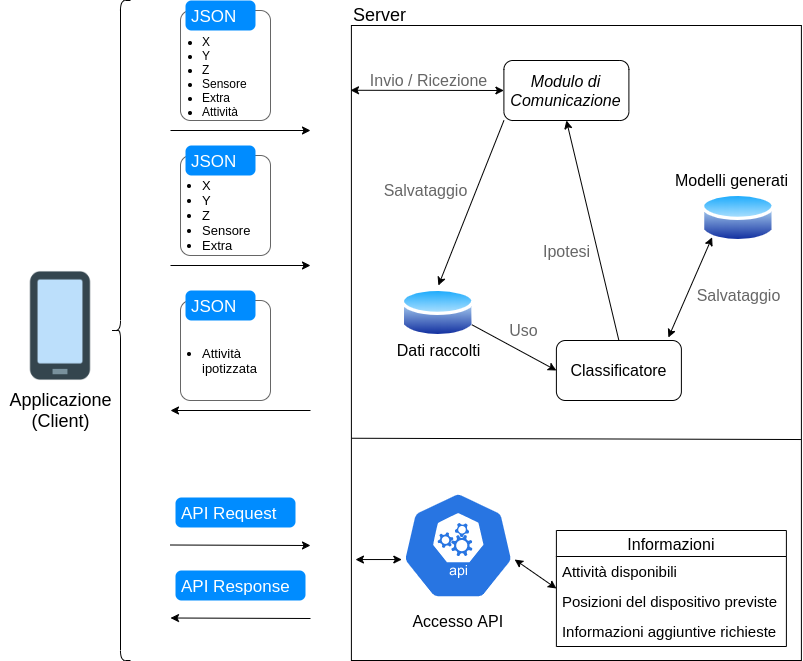
\includegraphics[scale = 0.41]{assets/images/overview.png}
    \caption{Panoramica del progetto}
\end{figure}

\subsubsection{Applicazione}
L'applicazione Android ha il compito di ottenere i dati relativi ai movimenti dell'utente 
e gestire lo scambio di tutte le informazioni raccolte con il server.
\subsubsection{Classificatore}
Il componente che effettuerà la classificazione, che come abbiamo detto, gestirà la mole di valori ottenuta tentando di 
eseguire il riconoscimento vero e proprio delle attività.
\subsubsection{Rest API}
Sono poi state aggiunte delle API Rest utilizzate come fonte iniziale di informazioni. Vedremo essere indispensabili 
per rendere l'intero sistema programmabile in modo dinamico, almeno per quanto riguarda tutto ciò che sarà impostabile 
da un amministratore in fase di avvio.